\section{\tech \protect\cat Approach }

\begin{figure}
    \centering
    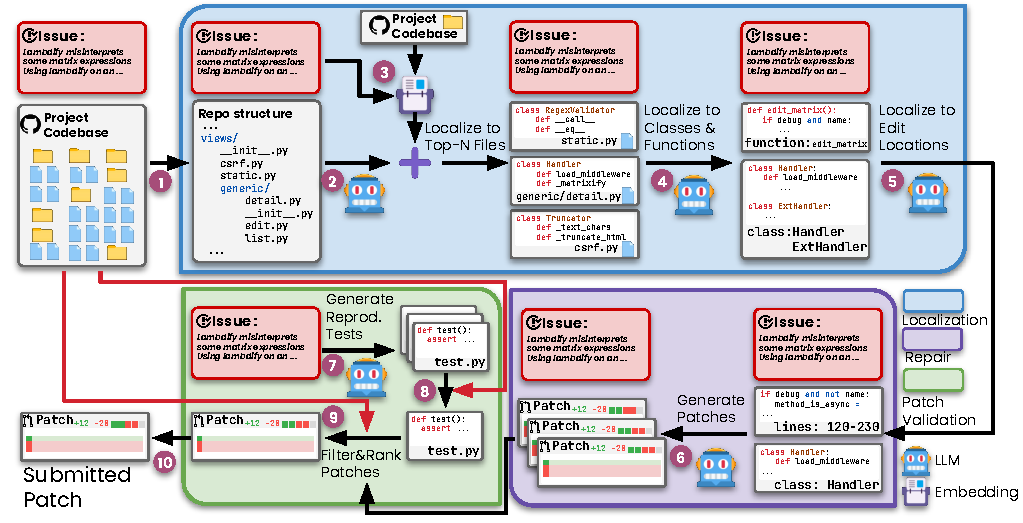
\includegraphics[width=1\columnwidth]{figs/overview.pdf}
    \caption{Overview of \tech.}
    \label{fig:overview}
\end{figure}


Figure~\ref{fig:overview} shows the overview of \tech, consisting of three phases: \textbf{localization}, \textbf{repair}, and \textbf{patch validation}. 
We first take in the issue description and the existing project codebase as input. 
Then, we begin our hierarchical localization process by turning the project codebase into a tree-like structure that {illustrates} the relative location of each file in the project \circled{1}.
Next, using this repository structure along with the original issue description, we {prompt} the \llm to localize and rank the top N most suspicious files that {likely require} editing to solve the issue \circled{2}. 
Since our repository structure format does not contain detailed source code information, we additionally retrieve files with most relevant code snippets with the issue description{ using embedding-based retrieval}  \circled{3}. 
We then combine the retrieved files with the \llm-localized files to obtain the final list of suspicious files. 
However, not all contents in each file need to be modified. 
As such, we provide a skeleton for each file (\ie a list of declaration headers of the classes and functions) and ask the \llm to output a specific list of classes and functions that we should examine more closely to fix the bug \circled{4}.
We then provide the complete code content of the previous locations and ask the \llm to finalize a smaller set of edit locations (\ie classes, functions, or even specific lines) \circled{5}.
For the repair phase, we provide the code snippets at these edit locations together with the issue description and {prompt} the \llm to sample multiple patches to solve the issue \circled{6}.
Next, we enter the patch validation phase, where we first ask the \llm to sample multiple \reproduction tests that aim to replicate the original issue \circled{7}, and then select the optimal one based on actual execution results on the original codebase \circled{8}. 
\tech uses the \reproduction test along with existing regression tests for patch ranking/selection \circled{9}.
Finally, \tech selects the top-ranked patch as the final patch for submission \circled{10}.
We now describe the steps in each of \tech{}'s phases in more detail. 


\subsection{Localization \protect\wearycat} 


To fix or implement a new feature, the first step is to obtain the locations in the source code, as without the correct locations, it can be impossible to provide the right edits. 
The difficulty lies in the fact that there could be hundreds of files
with thousands of lines of code each in a repository, whereas the correct locations to edit are only a few selected lines or functions.
\tech addresses this by using a simple three-step hierarchical localization process: 1) localize to {suspicious} files; 2) localize each selected files into relevant classes{, functions, and variables;} 3) localize to code edit locations.

\subsubsection{Localize to suspicious files.} 
\label{sec:localize_suspicious_files}
First, \tech narrows down potential locations to specific suspicious files. 
Instead of providing the complete code snippet for each file, \tech constructs {a concise representation of} the repository's file and directory structure, similar to the Linux \CodeIn{tree} command. 
We refer to this as the \textbf{\repostructureformat},
which begins with the root folder of the repository and organizes code files or folder names. 
Files and folders at the same directory level are aligned vertically, and files/folders in sub-directories are indented. 
We recursively traverse the entire repository to obtain the structure, which will be used as input for the \llm. 
The \repostructureformat provides the necessary file path{s alongside} the neighboring file names {}{to maintain organizational information in the original codebase}.
\tech then inputs the processed repository structure along with the original issue description to an \llm, and requests it to identify {a} list of the top N suspicious files{ that need {}{further inspection or} modification} to {resolve} the issue. 

To compliment the prompting-based localization (using file names only), \tech also uses a simple embedding-based retrieval method to {identify} additional suspicious files. 
However, instead of embedding all files in the repository, \tech first {filters out} irrelevant folders. 
This is done by providing the previously described repository structure and asking the \llm to produce a list of \emph{irrelevant} folders that do not need to be further inspected or modified to resolve the issue.
After removing all files from these irrelevant folders, \tech{} divides each remaining file into chunks of code segments and computes the embedding for each chunk using an embedding model. 
\tech then embeds the original issue description (i.e., the query) and computes the cosine similarity between the resulting query embedding and each chunk embedding to retrieve a list of relevant files that contain code segments with the highest similarity to the query. 
Finally, \tech combines the files obtained via prompting with those retrieved via embedding by selecting top N most common files localized by both, resulting in a final list of relevant files. 




\begin{wrapfigure}{r}{0.35\textwidth}
  \begin{center}
    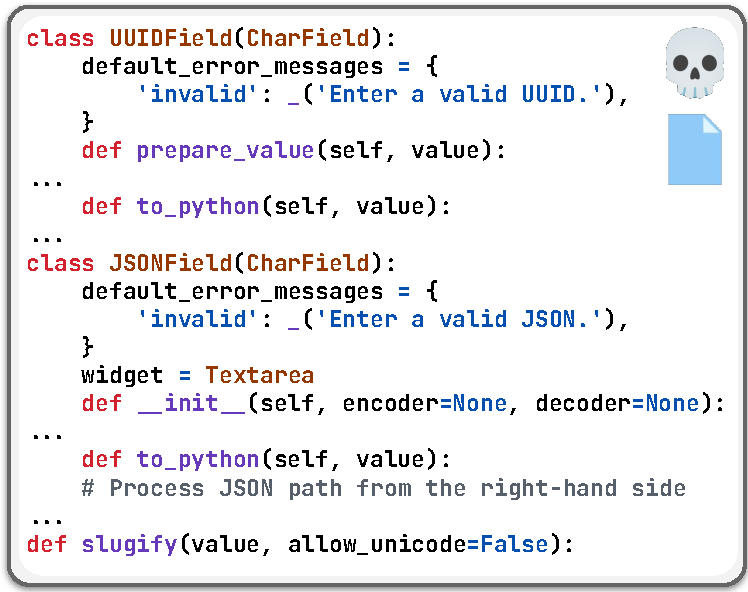
\includegraphics[width=0.35\textwidth]{figs/skeleton_file.pdf}
  \end{center}
  \caption{File skeleton format.}
  \label{fig:skeleton_example}
\end{wrapfigure}

\subsubsection{Localize to related elements.}
\label{sec:localize_related_elements}
After obtaining the list of suspicious files, \tech{} {proceeds} to the second part of the localization process: localize the related{ elements} within these files.
Directly providing the complete context of all files can be large.
As such, \tech builds a compressed format of each file that contains the list of class, function, or variable declarations.
We refer to this format as the \textbf{skeleton format}, with an example shown in Figure~\ref{fig:skeleton_example}. 
In the skeleton format, we provide only the {headers} of the classes and functions in the file.
For classes, we further include any class fields and methods (signatures only).
Additionally, we also keep comments in the class and module level to provide further information. 
%
Compared to providing the entire file context to the model, the skeleton format is a much more concise representation, especially when the file contains thousands of lines, making it impractical/costly to process all at once with existing \llm{s}.
We provide the skeleton of all suspicious files to the \llm at one time in a single prompt, enabling the model to comprehensively analyze the pertinent information and decide the most relevant elements.
Using this input, we prompt the \llm to provide a list of related classes and functions that one should examine to fix the provided issue.

\begin{wrapfigure}{r}{0.45\textwidth}
  \begin{center}
    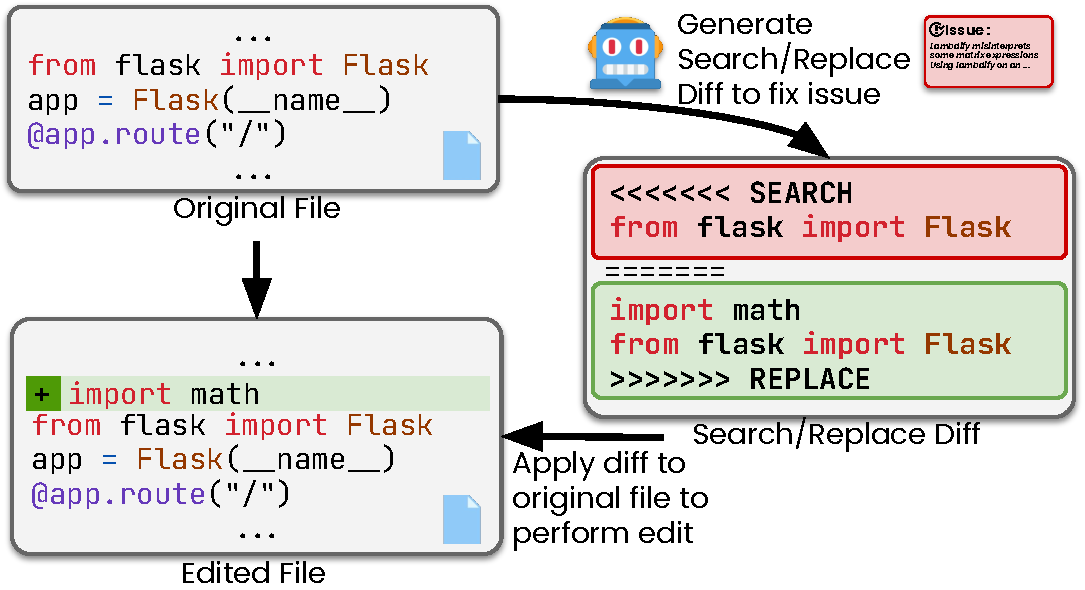
\includegraphics[width=0.45\textwidth]{figs/diff_format.pdf}
  \end{center}
  \caption{Search/Replace edit format.}
  \label{fig:diff_format}
\end{wrapfigure}

\subsubsection{Localize to edit locations.}
The previous localization step provided us with a list of related code elements; since we localize top N suspicious files, these localized related code elements could be from different files.
We now directly provide the code content from these elements to the \llm and ask it to localize specific edit locations.
Compared to using the entire file, the input context here is much smaller.
With this input, we then ask the \llm to identify the final set of edit locations{, specified by} line numbers, functions, or classes. 
Our simple hierarchical localization allows \tech to select a set of relevant code snippets as edit locations for repair{}.




\subsection{Repair \protect\smugcat}


In the repair stage, the goal is to produce the correct patch to solve the issue. 
Following existing work on \llm{}-based program repair~\cite{alpharepair, kolak2022patch, codexrepair, jiang2023study}, we first utilize the identified edit locations and construct a context window of code snippets to provide to the \llm for repair.
For example, if the identified location was a class from line 40 to 78, we would produce a context window of \CodeIn{[40 - x, 78 + x]} where \CodeIn{x} denotes the context window size. 
The intuition behind adding the additional code before and after the identified location is to provide the \llm with relevant contextual information for better program repair~\cite{alpharepair}. 
If multiple edit locations are identified, we would concatenate these context windows together separated with ``\CodeIn{...}'' to indicate missing context in the middle.

Using the code snippets, we then ask the \llm to generate patches to solve the issue.  
However, instead of directly producing the entire code snippet to replace the entire given context, \tech asks the \llm to generate a \textbf{Search/Replace edit}~\cite{aidar}: a simple 
diff format to efficiently create each patch. 
Figure~\ref{fig:diff_format} shows an example of the Search/Replace format containing two main parts: 1) search: the original code snippet we want to replace and 2) replace: the replacement code snippet we want to replace with.
To apply the generated Search/Replace diff to the original file, we can simply match the search code snippet and replace it with the replacement. 
This simple diff format avoids generating the complete code and instead focuses on producing small edits, which are not only more cost-efficient, but also more reliable and accurate (less chances for hallucination).
For each issue, \tech uses the \llm to generate multiple potential patches (starting with greedy and then sample multiple patches with higher temperature). 






 \subsection{Patch Validation \protect\grinningcat}

\begin{wrapfigure}{r}{0.4\textwidth}
  \begin{center}
    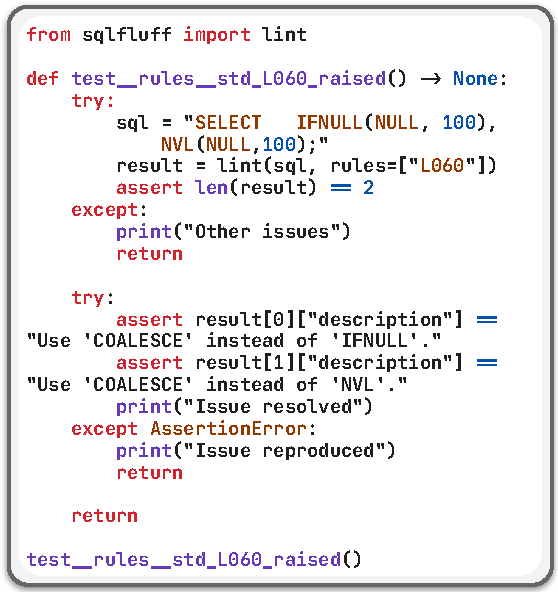
\includegraphics[width=0.4\textwidth]{figs/reproduction_test.pdf}
  \end{center}
  \caption{Example \reproduction test.}
  \label{fig:test}
\end{wrapfigure}

 \subsubsection{Reproduction test generation.} 
 \label{sec:reproduction_test_generation}
 Since \tech generates multiple candidate patches per issue, we need a way to select a final patch for submission.
 Please note that under the realistic \swebench setup, the original project codebase can only provide regression tests and not any \reproduction tests (i.e., bug-triggering tests). 
 This is because the issue has just been raised and the developers have not added any additional tests to trigger the issue.  
 As such, different from the Generate-and-Validate program repair setup~\cite{long2016analysis}, we do not have access to bug-triggering tests. %
%

Following prior work~\cite{specrover, coder}, \tech generates additional \reproduction test to help with patch selection. More specifically, \tech leverages the \llm to synthesize a complete testing file that attempts to both reproduce the original issue described in the issue description, as well as verify whether the issue has been fixed.
 Figure~\ref{fig:test} shows an example of the \reproduction test that we want the model to synthesize. 
 {If the issue is reproduced}, the test outcome should print \CodeIn{Issue reproduced}. 
 On the other hand, the test should output \CodeIn{Issue resolved} if the issue has been fixed. 
 We also include another output of \CodeIn{Other issues} if the test runs into any unexpected issues. 
 To generate the \reproduction test, \tech provides the original issue description with an example \reproduction test to demonstrate the test format.
 Similar to repair, we also sample multiple candidate \reproduction tests and then execute each test on the original repository to filter any tests that do not output \CodeIn{Issue reproduced}. 
 Finally, we normalize each test (remove comments, extra spaces, and normalize test names) and then select the test with the highest number of occurrence as the final \reproduction test for each issue.


\subsubsection{Patch selection.} 
\label{sec:patch_filtering}

Using the generated \reproduction tests, we start our patch selection process to pick the final submission patch.
%
\tech first runs all the existing tests in the repository to identify a set of passing tests that successfully pass in the original codebase. 
However, not all of those passing tests should be considered as regression tests since solving the issue may require changing some of the existing functionalities. 
Therefore, \tech provides the list of passing tests to the \llm and ask it to identify any tests that should not be ran to check if the issue has been correctly fixed (\ie the tests that may be updated/patched during issue fixing). 
After removing the \llm-identified non-regression tests, we obtain a final set of regression tests. 
We then run the set of regression tests on all the generated patches. 
\tech then keeps the patches with the lowest number of regression failures.
For those patches, \tech then runs the selected \reproduction test and only keeps patches that output \CodeIn{Issue resolved}.
Meanwhile, because the \reproduction test is generated by the \llm and can potentially be incorrect/imprecise, it could be possible that no patch can pass the \reproduction test; in that case, \tech will fall back on only using the regression test results for selection.
\tech then applies a re-ranking approach using majority voting:
We first normalize each patch to ignore surface-level differences (\eg extra spaces, newlines, and comments), and then select the patch with the highest number of occurrences as the final patch for submission. 
More specifically, to standardize the patch, we begin by parsing both the old and new code (after applying the patch) into abstract syntax trees. Next, we unparse the trees into a canonical source code format with docstrings removed. Finally, we compute the textual diff between the standardized old and new code to get the normalized patch.

\tech solves repository-level issues using a simple step-by-step procedure.
We note here that none of the techniques used by \tech in isolation are{ revolutionary},
but instead \tech smartly combines existing techniques to construct an easy-to-understand approach. 
Different from prior autonomous agent-based tools that involve complex interactions with the environment, \tech uses{ a simplistic} three-phase approach to localize, repair, and validate without relying on any agents for decision-making.
By conducting localization in a hierarchical manner, \tech can efficiently and effectively compute the fine-grained locations for editing. 
\tech then performs repair by sampling multiple patches using a simple diff format.
\tech's patch validation approach can further aid the patch selection process by producing \reproduction tests that can help verify if the issue is fixed. 


